% !TEX options=--shell-escape
\pdfobjcompresslevel=0
\documentclass[slidetop,11pt]{beamer}
\usepackage[utf8]{inputenc}
\usepackage{dsfont}
\usepackage{multirow}
\usepackage{array}
\usepackage{xcolor}
\usepackage{algorithmic}
\usepackage[plain]{algorithm}
\usepackage{ulem}
\usepackage{mathabx}
\usepackage{graphicx}
% declare the path(s) where your graphic files are
\graphicspath{{img/}}
\DeclareGraphicsExtensions{.pdf,.jpeg,.png,.eps}
\usepackage{subfig}
\usepackage{soul} % strikethrough
\usepackage{minted}


\usetheme{progressbar}
\setbeamertemplate{footline}[frame number]
\setbeamercovered{transparent}
\useinnertheme{default}

\newcommand{\mv}{{\rm  MV}}

\DeclareMathOperator*{\argmin}{\arg\!\min}
\DeclareMathOperator*{\sgn}{\text{sgn}}

\newtheorem{prop}{Property}
\newtheorem{thm}{Theorem}
\newtheorem{rem}{Remark}

\newenvironment{changemargin}[2]{%
  \begin{list}{}{% 
    \setlength{\topsep}{0pt}% 
    \setlength{\leftmargin}{#1}% 
    \setlength{\rightmargin}{#2}% 
    \setlength{\listparindent}{\parindent}% 
    \setlength{\itemindent}{\parindent}% 
    \setlength{\parsep}{\parskip}% 
  }% 
  \item[]}{\end{list}}

\makeatletter
\newcommand{\vast}{\bBigg@{3}}
\makeatother
	
\definecolor{dgreen}{rgb}{0.,0.6,0.}
\definecolor{azure}{rgb}{0.,0.5,1.}
\definecolor{bluegray}{rgb}{0.4,0.6,0.8}
\definecolor{bleu}{rgb}{0.19,0.55,0.91}

\newcommand{\semitransp}[2][30]{\color{fg!#1}#2}


\title{{\large Anomaly detection in scikit-learn} \\ {\normalfont \small{Ongoing work and future developments}}}
\author{Albert Thomas}
\institute{T\'el\'ecom ParisTech - Huawei Technologies}


\begin{document}

\captionsetup[subfigure]{labelformat=empty}

\begin{frame}

\includegraphics[width=2.3cm]{img/scikit-learn-logo-notext.png}
% \hspace{6.7cm}
% \includegraphics[width=1cm]{img/logo_telecom.jpg}
\titlepage

\end{frame}


\begin{frame}
\frametitle{Anomaly detection}

\only<1-3>{
\begin{itemize}
\item \textbf{Imbalanced classification}: anomalies and normal data available
\end{itemize}
}

\visible<2->{
\begin{itemize}
\item \textbf{Novelty detection}: only normal data available
\begin{center}
fit on normal data, predict on unlabeled data
\end{center}
\end{itemize}
}

\visible<3->{
\begin{itemize}
\item \textbf{Outlier detection}: unlabeled data only,
\begin{center}
fit \textbf{and} predict on unlabeled data
\end{center}

Outliers are rare events, located in the low density regions.
\end{itemize}
}

\end{frame}


\begin{frame}\frametitle{Anomaly detection}
    
\begin{itemize}
\item \textbf{Novelty detection}: only normal data available
\begin{center}
fit on normal data, predict on unlabeled data
\end{center}
\item \textbf{Outlier detection}: unlabeled data only,
\begin{center}
fit \textbf{and} predict on unlabeled data
\end{center}

Outliers are rare events, located in the low density regions.
\end{itemize}
\begin{center}
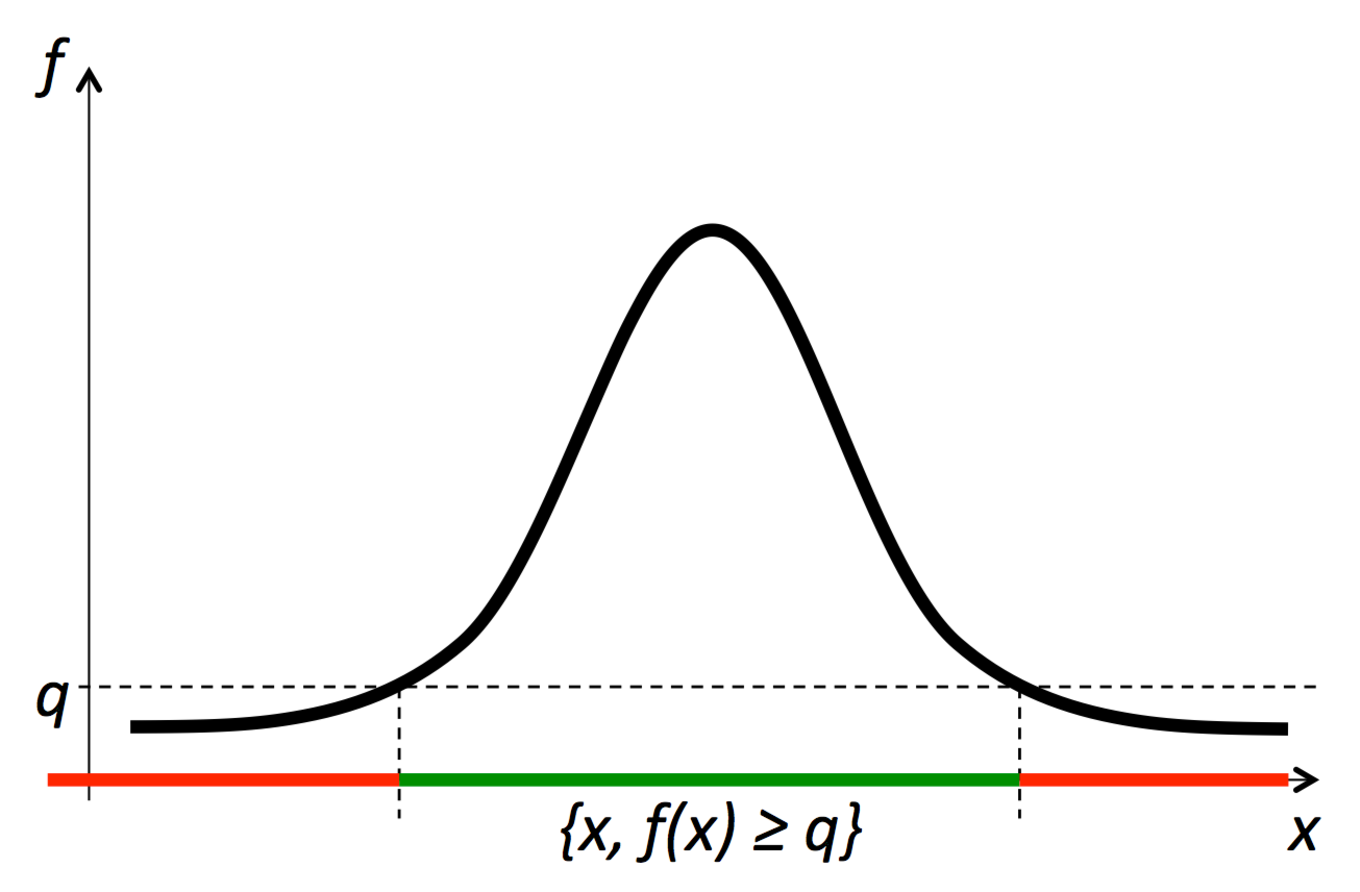
\includegraphics[width=7cm]{dls3.pdf}
\end{center}

\end{frame}


\begin{frame}
\frametitle{Outlier and novelty detection algorithms}

Common approach

\vspace{0.5cm}

\begin{enumerate}
\item[1.] Learn a scoring function $s$ such that
\begin{center}
the smaller $s(x)$ the more abnormal is $x$
\end{center}

\vspace{0.5cm}

\item[2.] Threshold $s$ at an offset $q$: outlier/novelties are such that
\begin{equation*}
\{x, s(x) < q \}
\end{equation*}
$q$ usually depends on a \mintinline{python}{contamination} parameter
\end{enumerate}

\begin{center}
EllipticEnvelope, OneClassSVM \\
IsolationForest (iForest) and LocalOutlierFactor (LOF)
\end{center}

\end{frame}


\begin{frame}[plain]\frametitle{Outlier Detection}
    
\begin{center}
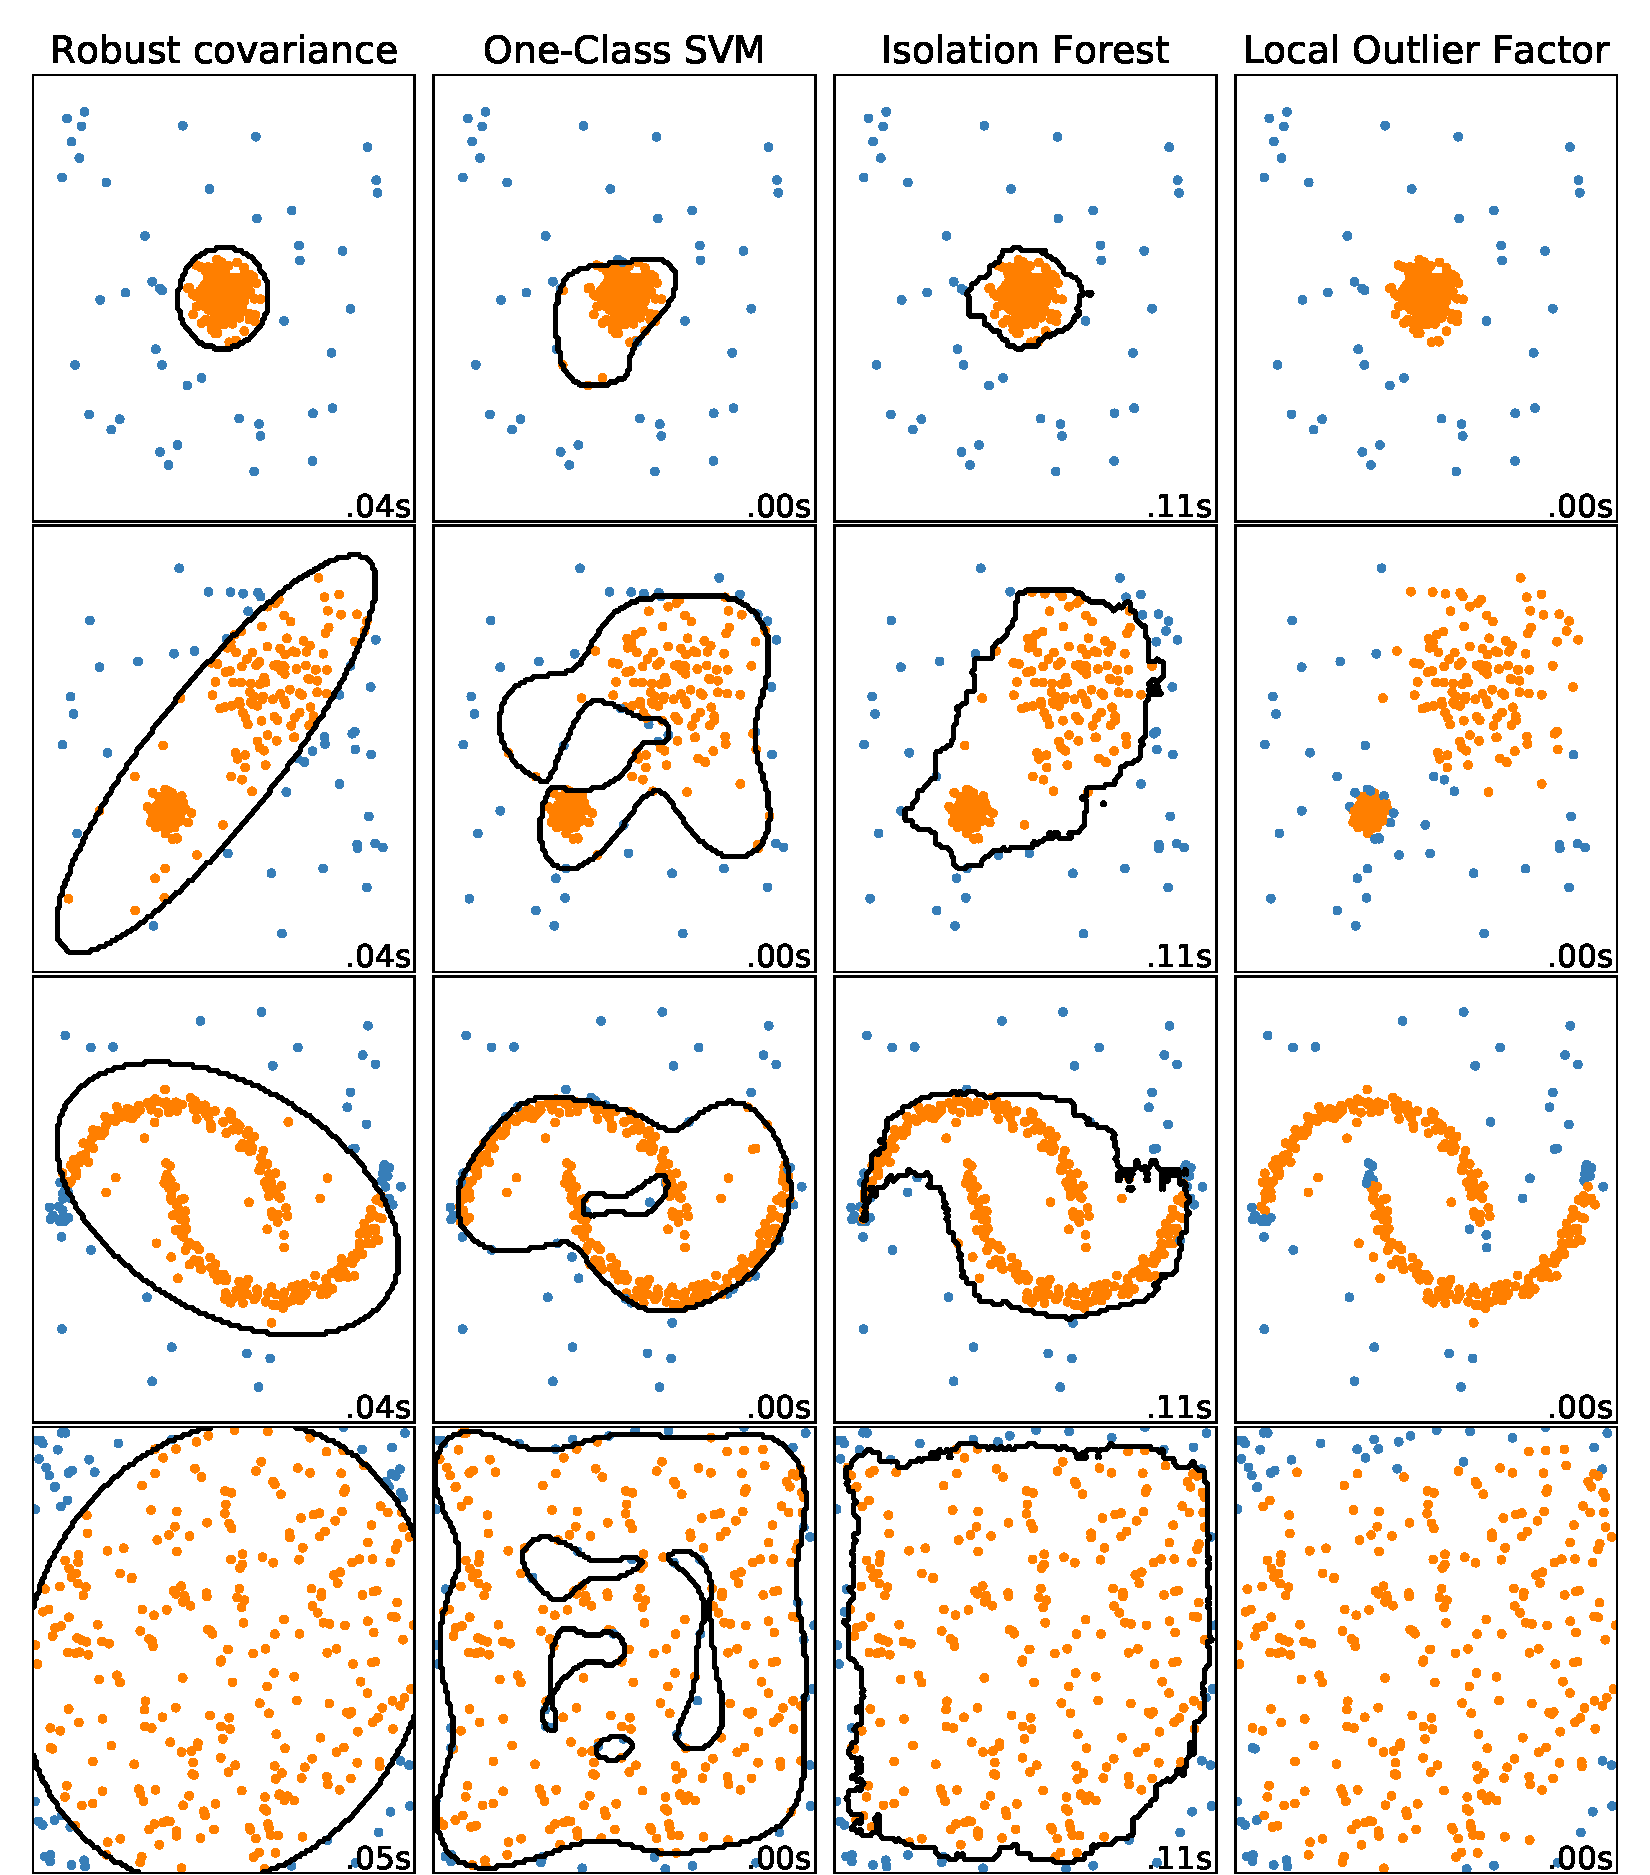
\includegraphics[width=7cm]{img/anomaly_comparison.pdf}
\end{center}

\end{frame}


\begin{frame}[plain]\frametitle{Local Outlier Factor}

\begin{center}
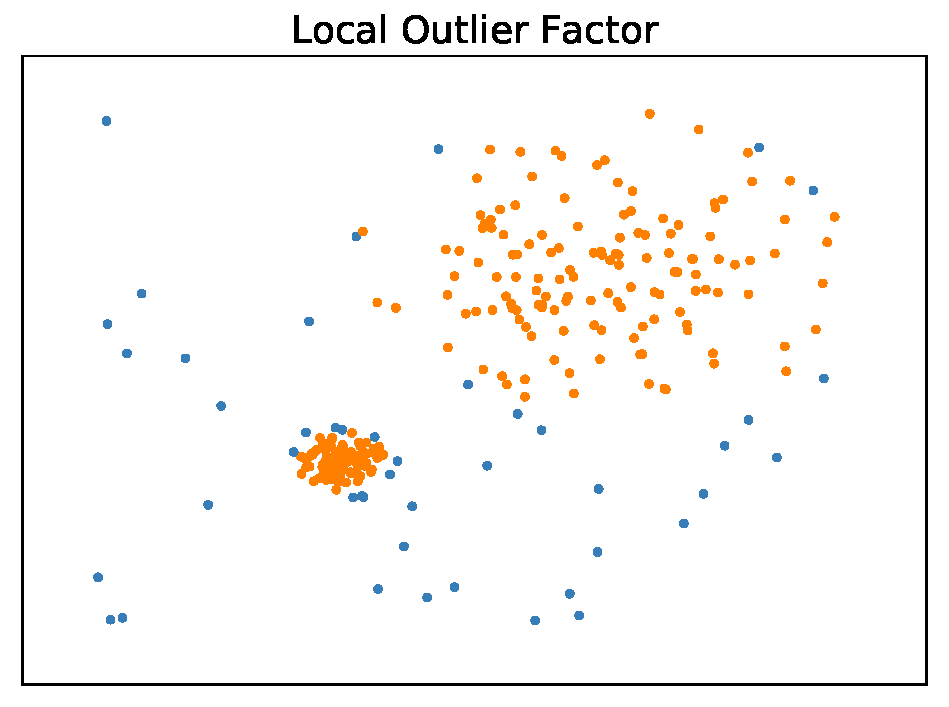
\includegraphics[width=7cm]{img/locality_lof.pdf}
\end{center}

\end{frame}


\begin{frame}[plain]\frametitle{Novetly detection}
    
\begin{center}
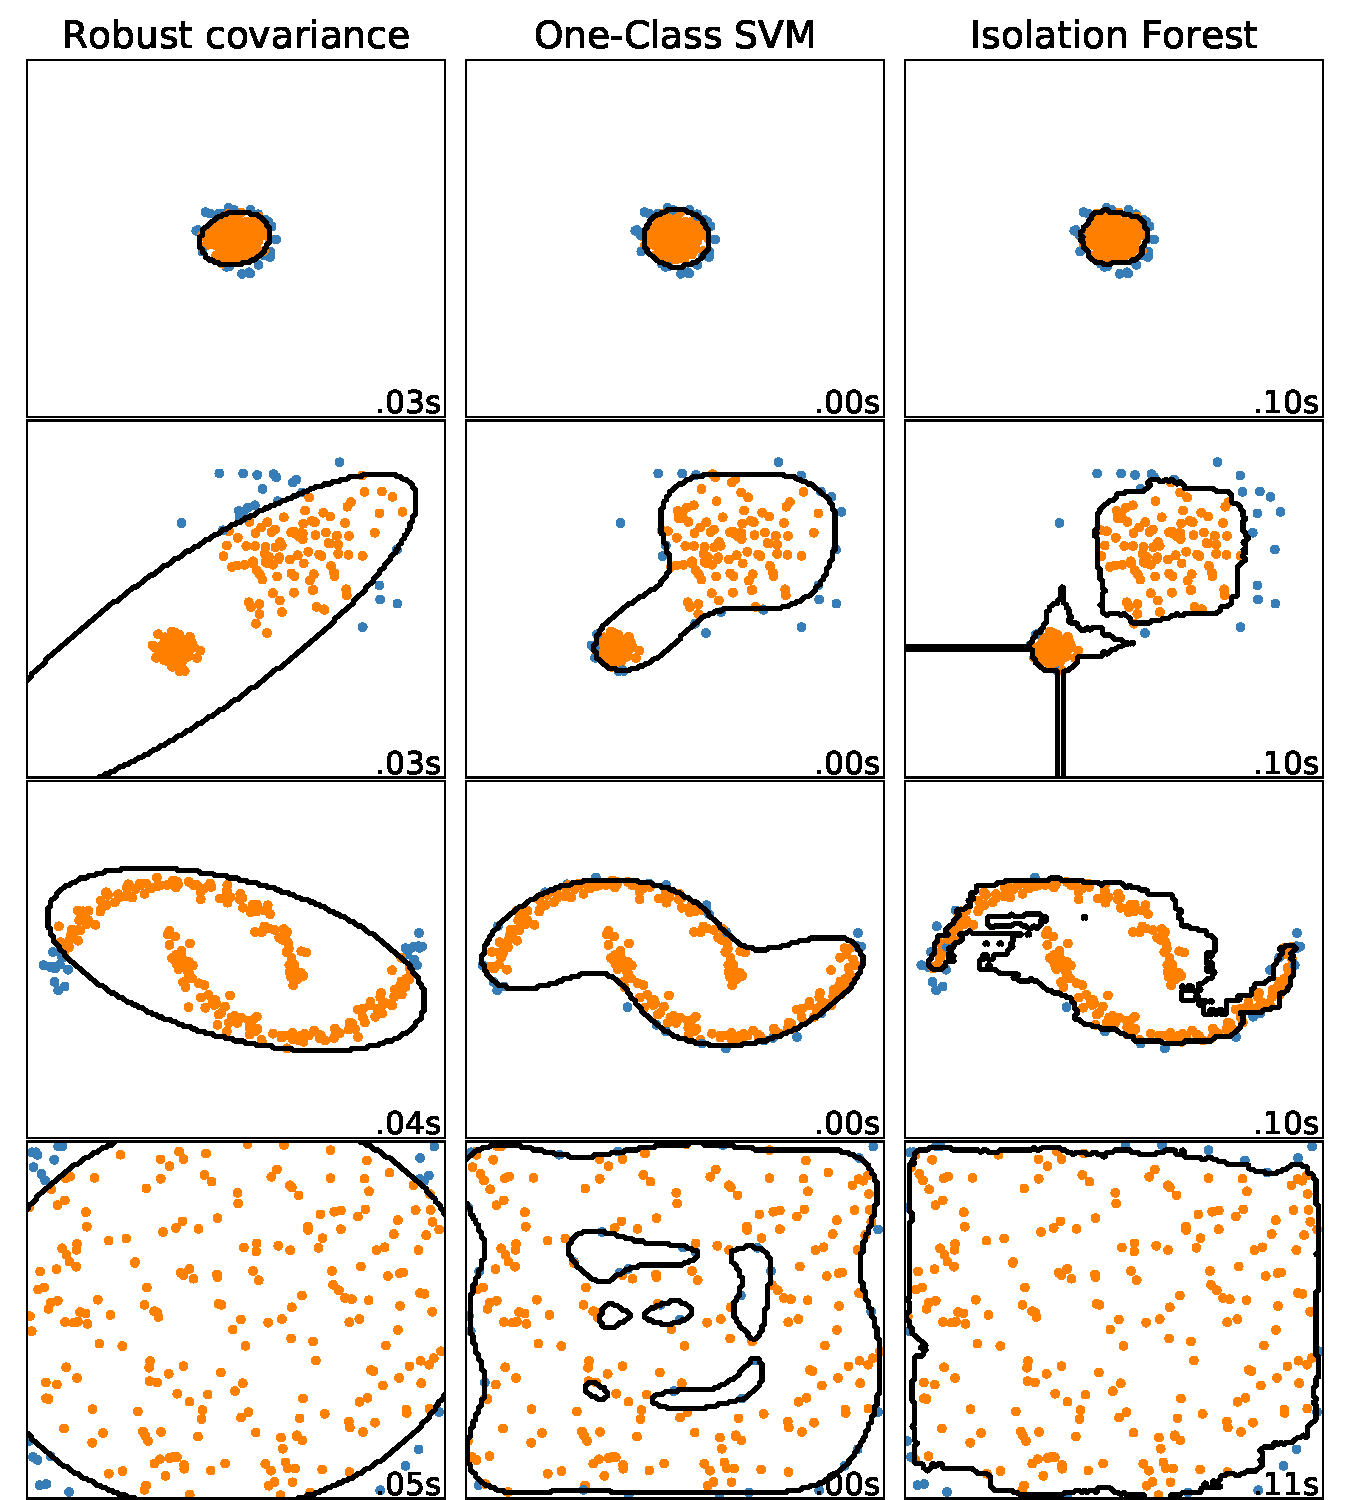
\includegraphics[width=7cm]{img/novelty_comparison.pdf}
\end{center}

\end{frame}


\begin{frame}[plain]
    
\begin{center}
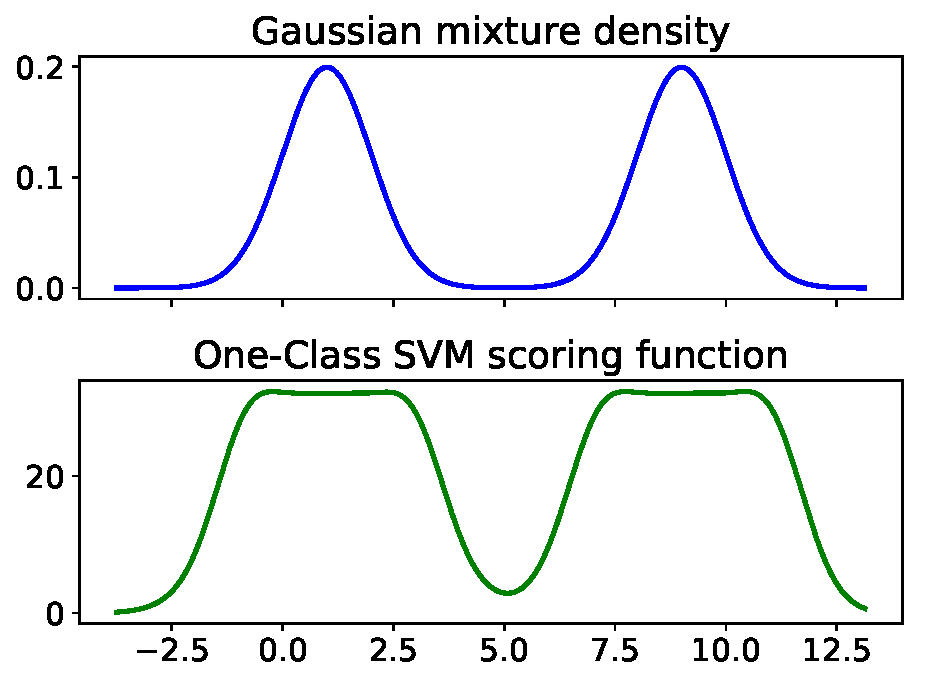
\includegraphics[width=9cm]{img/ocsvm_1d.pdf}
\end{center}

\end{frame}


\begin{frame}\frametitle{Scikit-learn API}
    
\begin{center}
PR on \textbf{API consistency} $\vcenter{\hbox{
\includegraphics[width=1.7cm]{img/merged_logo.pdf}}}$ last week
\end{center}

\begin{itemize}
  \item same \mintinline{python}{decision_function} for all estimators
  \vspace{0.5cm}
  \item new \mintinline{python}{score_samples} method
\end{itemize}

\end{frame}


\begin{frame}\frametitle{Scikit-learn API}

EllipticEnvelope, OneClassSVM and IsolationForest

\onslide<1->{
\begin{itemize}
  \item instantiate your estimator, e.g.~\mintinline{python}{clf = OneClassSVM()}
  \item \mintinline{python}{clf.fit(X_train)}
  \item \mintinline{python}{clf.score_samples(X_test)}: raw score $s$
  \item \mintinline{python}{clf.decision_function(X_test)}: thresholded score
  \begin{equation*}
  \mintinline{python}{clf.score_samples(X_test) - clf.offset_} \quad
  \begin{cases}
    \geq 0 \quad \text{for inliers} \\
    < 0 \quad \text{for outliers}
  \end{cases}
  \end{equation*}
  \item \mintinline{python}{clf.predict(X_test)}
  \begin{equation*}
  \begin{cases}
    +1 \quad \text{for inliers} \\
    -1 \quad \text{for outliers}
  \end{cases}
  \end{equation*}
\end{itemize}
}

\visible<2>{
\begin{center}
\alert{Not valid for LOF}
\end{center}
}

\end{frame}


\begin{frame}\frametitle{Scikit-learn API - Outlier detection}

LOF is based on $k$-NN distances

\vspace{0.5cm}

\begin{itemize}
  \item predict on $x \in X_{train}$: take the $k$ nearest neighbors of $x$ in $X_{train} \setminus \{x\}$
  \vspace{0.5cm}
  \item predict on $x \notin X_{train}$: take the $k$ nearest neighbors of $x$ in $X_{train}$
\end{itemize}

\vspace{0.5cm}

\begin{center}
Hard to check whether $x \in X_{train}$ or not...
\end{center}

\end{frame}


\begin{frame}\frametitle{Scikit-learn API - Outlier detection}

\onslide<1->{
1st solution
\vspace{0.5cm}
\begin{itemize}
  \item \mintinline{python}{fit_predict(X_train)} to predict on \mintinline{python}{X_train}
  \vspace{0.5cm}
  \item \mintinline{python}{predict(X_test)} to predict on \mintinline{python}{X_test}
\end{itemize}
}

\visible<2>{
\vspace{0.5cm}
\begin{center}
\alert{\mintinline{python}{fit(X).predict(X) != fit_predict(X)}}
\end{center}
}



\end{frame}



\begin{frame}\frametitle{Scikit-learn API - Outlier detection}

\onslide<1->{
2nd solution and current one
\vspace{0.3cm}
\begin{itemize}
  \item only \mintinline{python}{fit_predict} is public
  \vspace{0.3cm}
  \item \mintinline{python}{_score_samples}, \mintinline{python}{_decision_function} and \mintinline{python}{_predict} are private
\end{itemize}
% LOF's original paper is only about outlier detection
}

\visible<2->{
\vspace{0.3cm}
\begin{center}
\textbf{Novelty detection is not (officially) supported for LOF}
\end{center}
\vspace{0.3cm}
\begin{center}

\includegraphics[width=1.8cm]{img/shocking.jpg}
\end{center}
}

\end{frame}


\begin{frame}\frametitle{Scikit-learn API}

\mintinline{python}{contamination} parameter in $(0, 1)$ / \mintinline{python}{nu} for OneClassSVM

\vspace{0.3cm}

\begin{itemize}
  \item for outlier detection: proportion of outliers in the data set
  \vspace{0.3cm}
  \item for novelty detection: type-I error (false positive rate)
\end{itemize}

\vspace{0.5cm}

Used to compute the offset $q$ on the training set
\begin{equation*}
\{s(x) < q \} = \{\text{\mintinline{python}{clf.score_samples(x) < clf.offset_}}\}
\end{equation*}

\end{frame}


\begin{frame}\frametitle{Scikit-learn API}

\mintinline{python}{contamination} can be set to \mintinline{python}{'auto'} for iForest and LOF
\vspace{0.4cm}
\begin{itemize}
  \item iForest: score of inliers close to 0 and score of outliers close to -1
  \begin{equation*}
  \mintinline{python}{clf.offset_ = -0.5}
  \end{equation*}
  \vspace{0.2cm}
  \item LOF: score of inliers $\approx -1$
  \begin{equation*}
  \mintinline{python}{clf.offset_ = -1.5}
  \end{equation*}
\end{itemize}

\end{frame}


\begin{frame}\frametitle{Common tests}

$\vcenter{\hbox{
\includegraphics[width=1.4cm]{img/open_logo.pdf}}}$ PR on \textbf{common tests for outlier detection estimators}

\vspace{0.5cm}

\begin{itemize}
  \item Create an \mintinline{python}{OutlierMixin}
  \begin{center}
  defines a \mintinline{python}{fit_predict} for all outlier and novelty detection estimators
  \end{center}
  \vspace{0.4cm}
  \item For all estimators test \mintinline{python}{fit_predict}
  \vspace{0.5cm}
  \item For novelty detection estimators test \mintinline{python}{score_samples}, \mintinline{python}{decision_function}, \mintinline{python}{offset_}
\end{itemize}
  

\end{frame}


\begin{frame}[fragile]\frametitle{OneClassSVM with SGD}

$\vcenter{\hbox{
\includegraphics[width=1.4cm]{img/open_logo.pdf}}}$ PR on \textbf{OneClassSVM using SGD}

\begin{itemize}
  \item Solves a linear version of the OneClassSVM
  \item Pipeline with a kernel approximation
\end{itemize}

\vspace{0.5cm}

\begin{minted}{python}

  from sklearn.kernel_approximation import Nystroem
  from sklearn.linear_model import SGDOneClassSVM

  nystroem = Nystroem(gamma=gamma)
  online_ocsvm = SGDOneClassSVM(nu=nu)
  pipe_online = make_pipeline(nystroem, online_ocsvm)

  pipe_online.fit(X_train)

\end{minted}

\end{frame}


\begin{frame}[plain]

% $\vcenter{\hbox{
\includegraphics[width=1.4cm]{img/open_logo.pdf}}}$ PR on \textbf{OneClassSVM using SGD}
\begin{changemargin}{-0.5cm}{+1.cm}
\only<1>{
\begin{center}
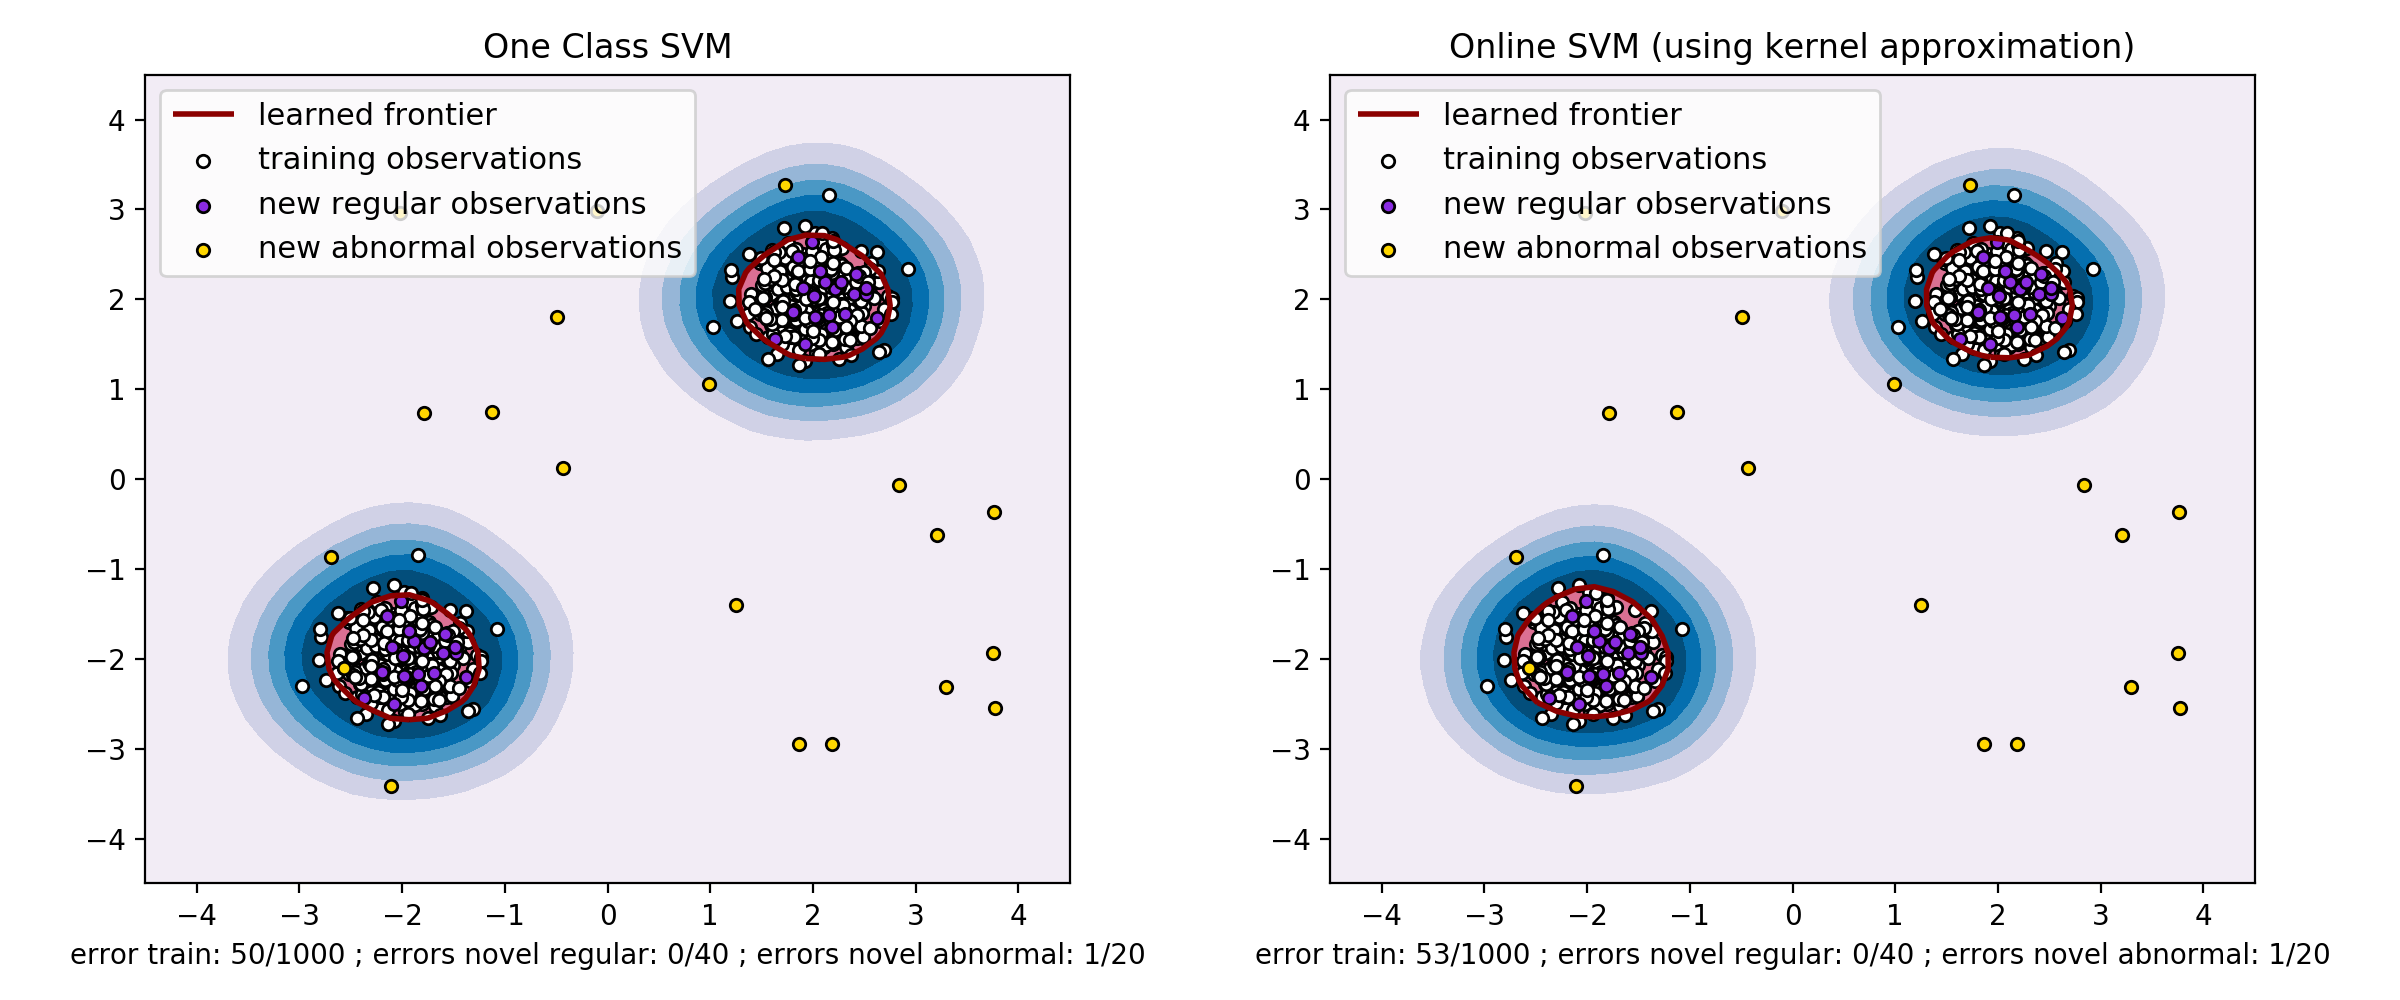
\includegraphics[width=12cm]{img/example_sgdocsvm.png}
\end{center}
}

\only<2>{
\begin{center}
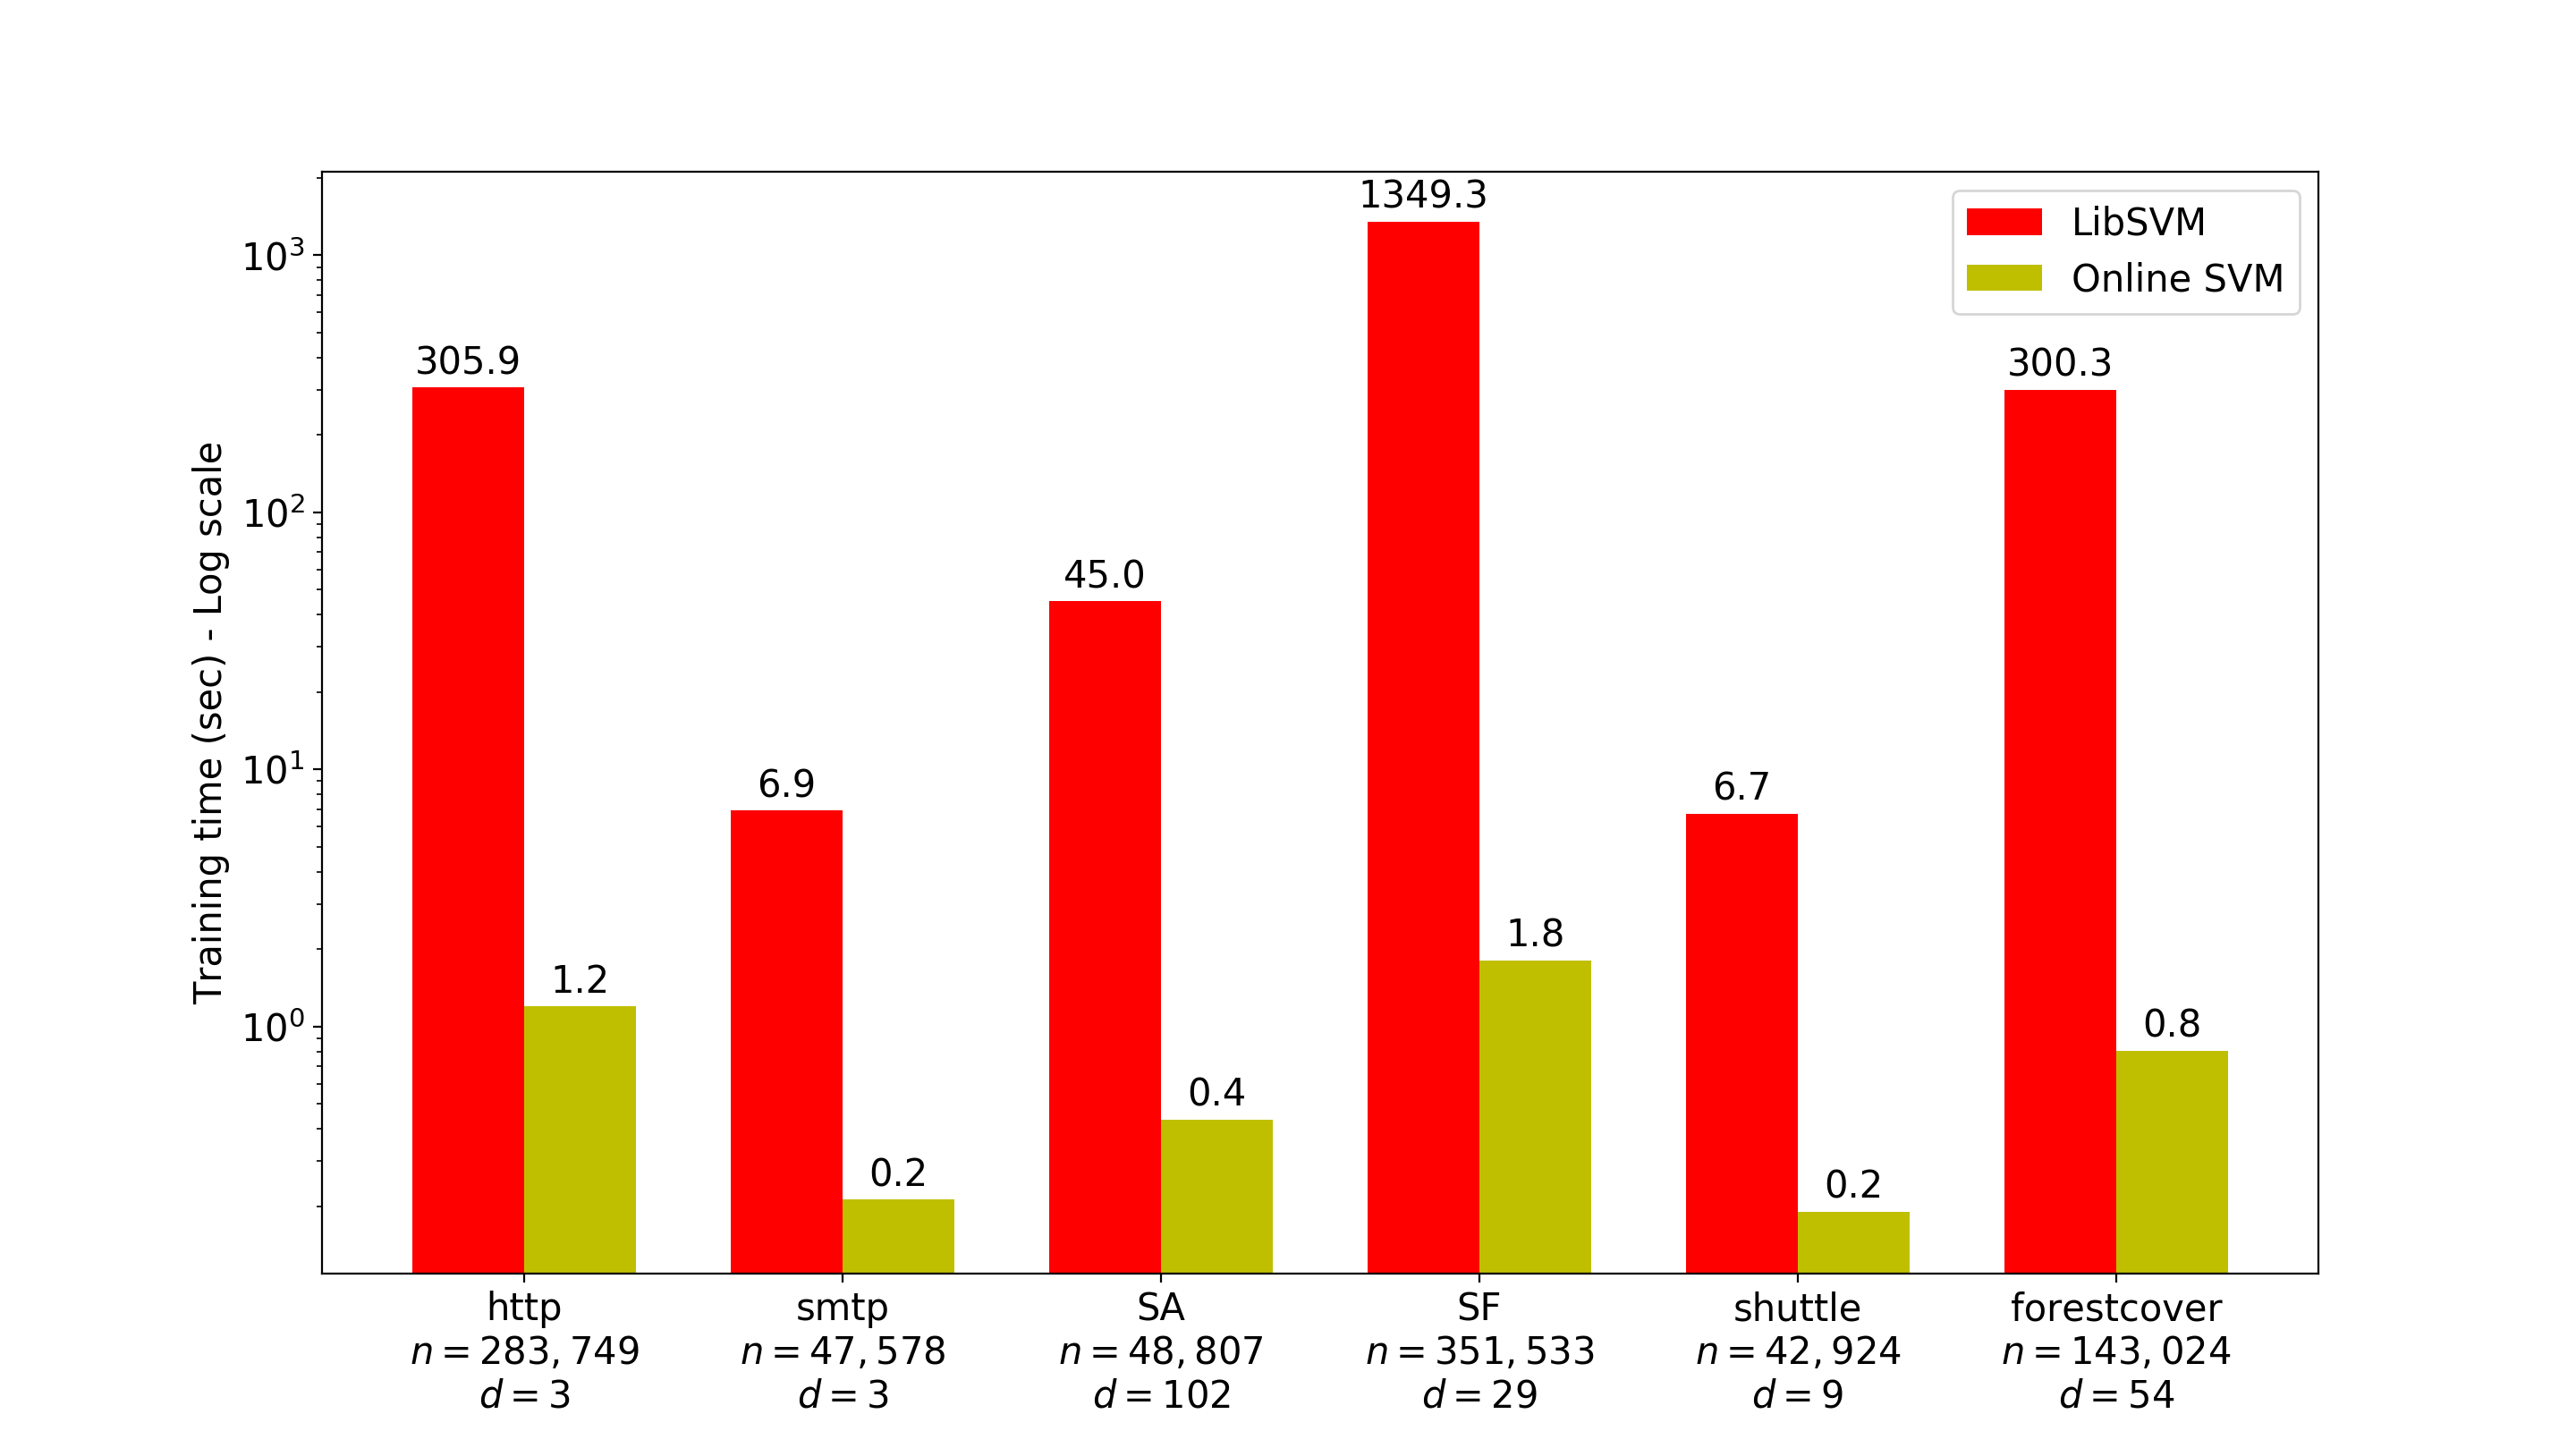
\includegraphics[width=12cm]{img/time_sgdocsvm.png}
\end{center}
}

\only<3>{
\begin{center}
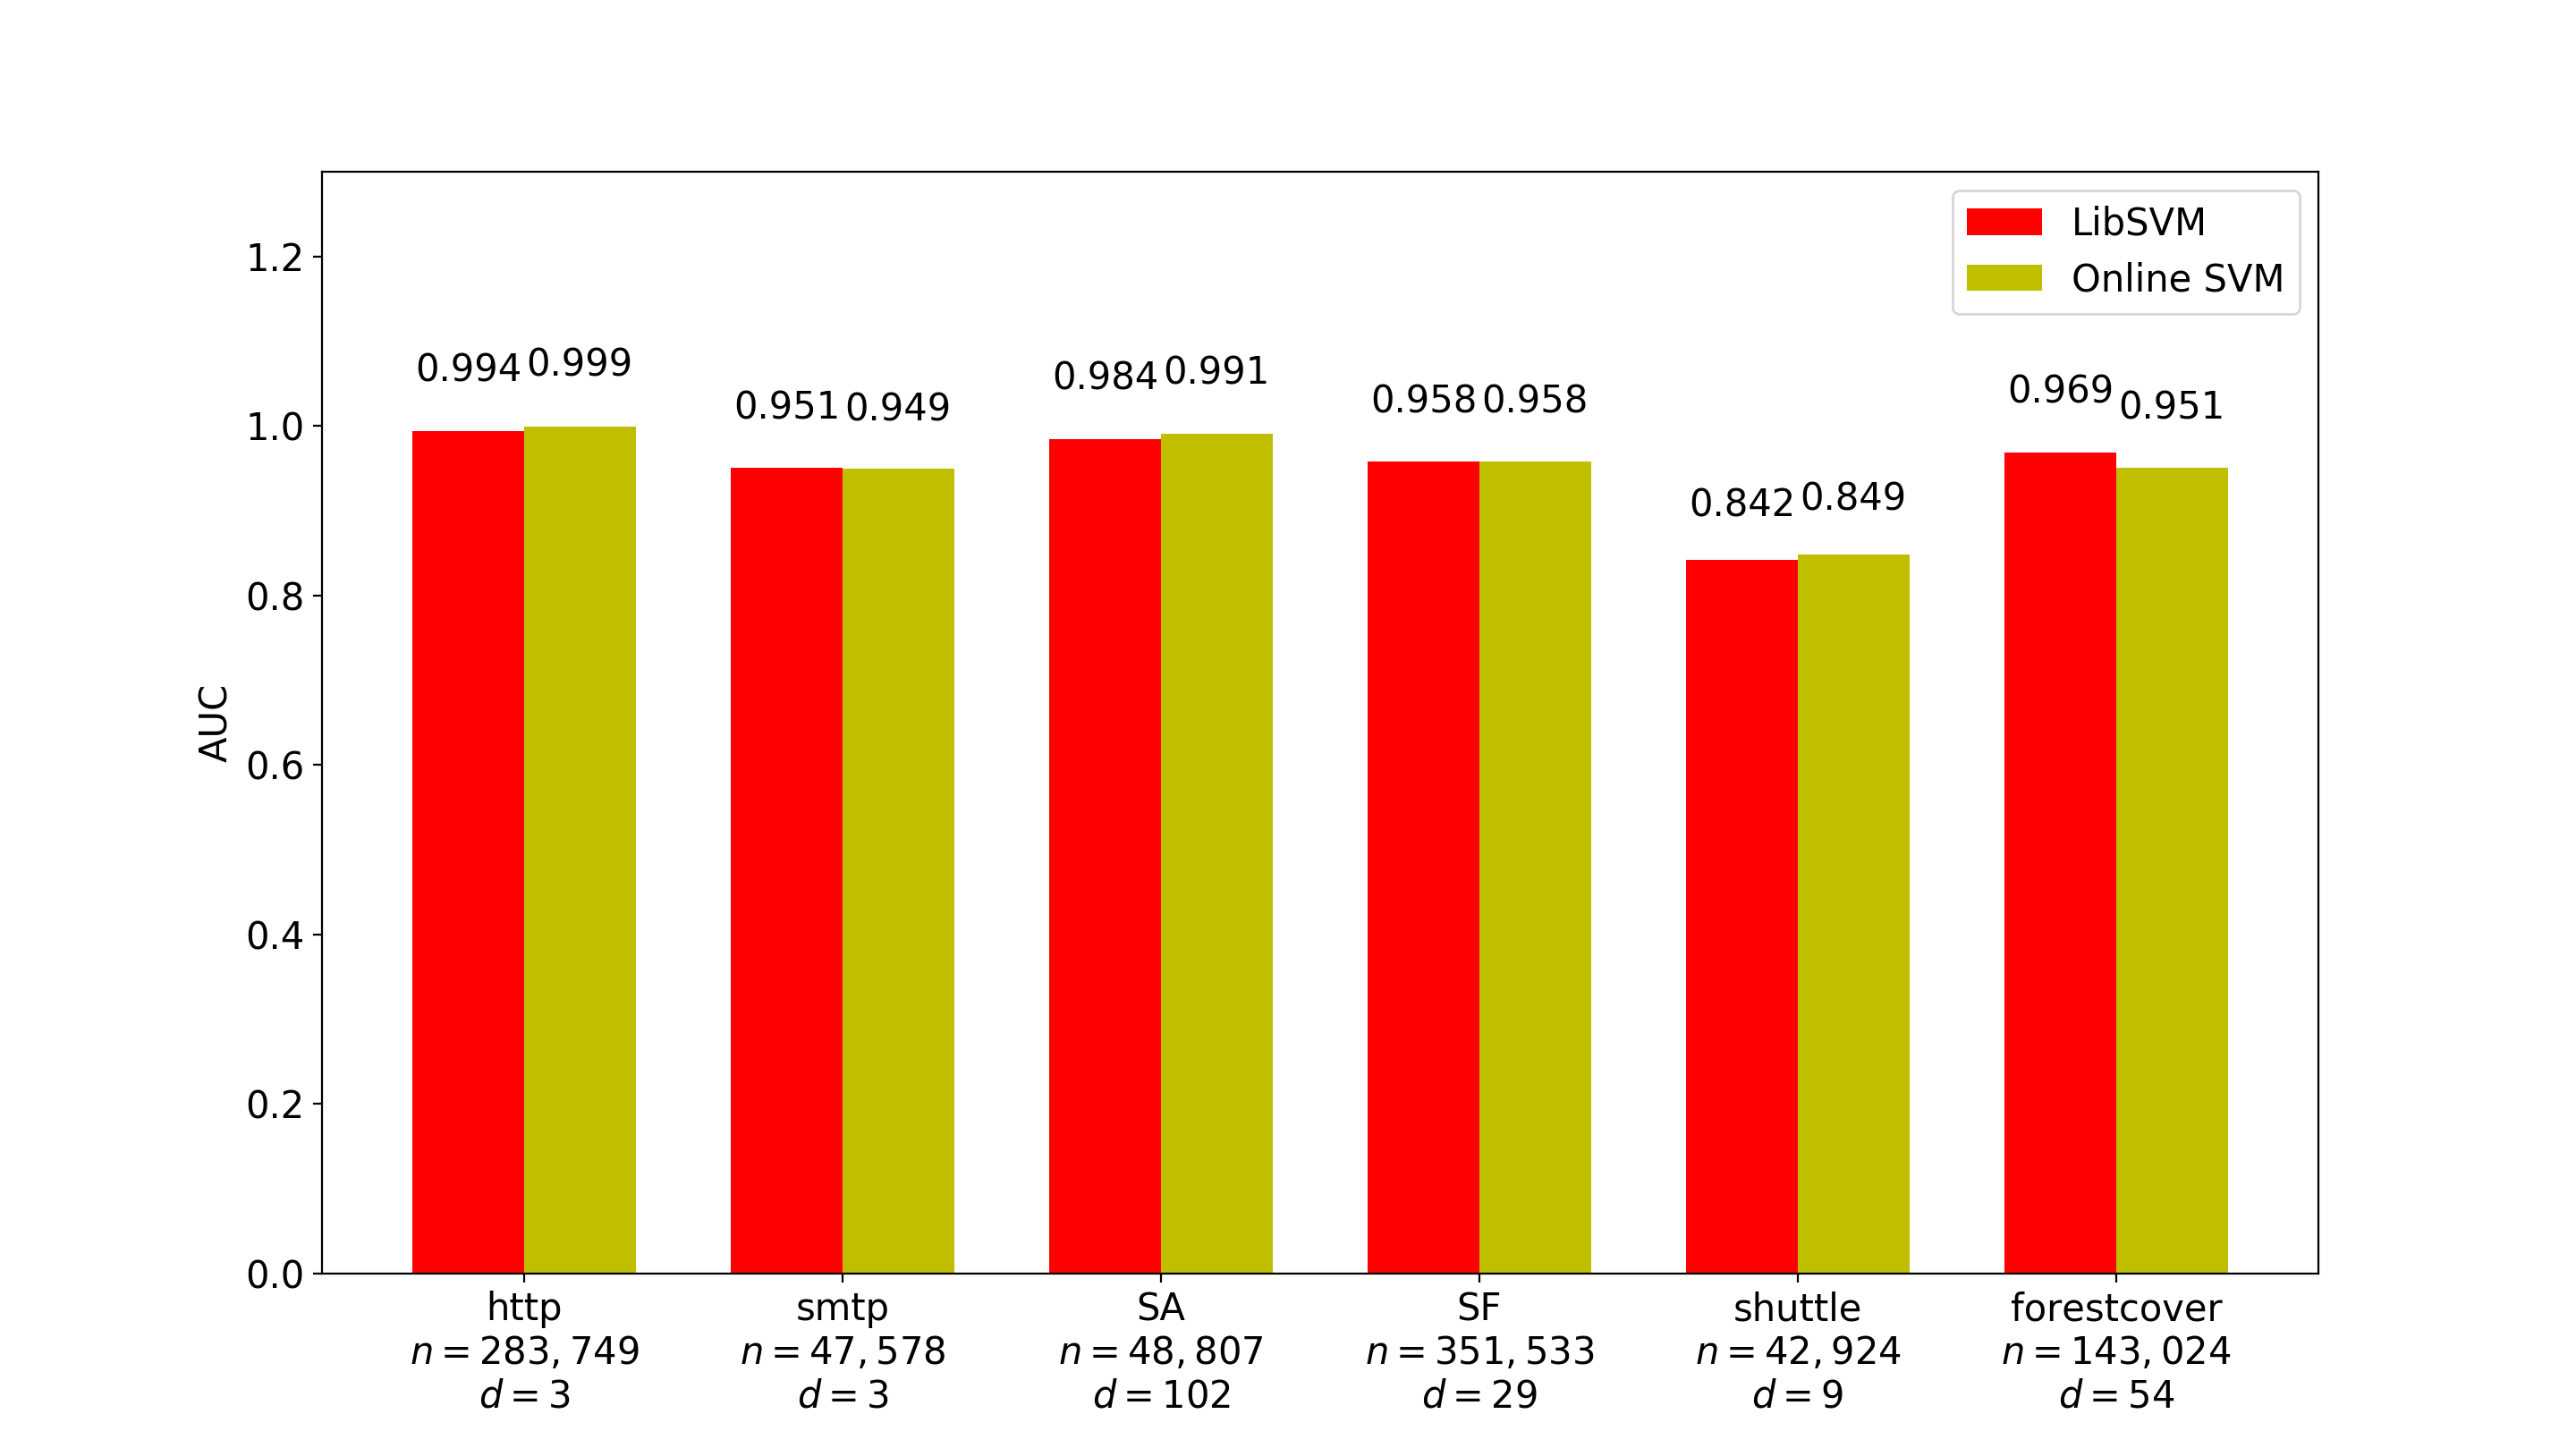
\includegraphics[width=12cm]{img/auc_sgdocsvm.png}
\end{center}
}
\end{changemargin}

\end{frame}

\renewcommand{\arraystretch}{1.5}

\begin{frame}\frametitle{Future work}

Novelty detection for LOF
\begin{center}
add \mintinline{python}{novelty} parameter in \mintinline{python}{__init__}
\end{center}


\begin{itemize}
  \item \mintinline{python}{novelty=False} (default)
\end{itemize}
{\footnotesize
  \begin{center}
  \begin{tabular}{ | c | c | }
    \hline
    \mintinline{python}{fit_predict} & \mintinline{python}{predict}/\mintinline{python}{decision_function}/\mintinline{python}{scores_samples}\\ \hline
    OK & \mintinline{python}{NotImplementedError} \\ \hline 
  \end{tabular}
\end{center}
}


\begin{itemize}
  \item \mintinline{python}{novelty=True}
\end{itemize}
{\footnotesize
  \begin{center}
  \begin{tabular}{ | c | c | }
    \hline
    \mintinline{python}{fit_predict} & \mintinline{python}{predict}/\mintinline{python}{decision_function}/\mintinline{python}{scores_samples}\\ \hline
    \mintinline{python}{NotImplementedError} & OK \\ \hline 
  \end{tabular}
\end{center}
}

\end{frame}




% \begin{frame}\frametitle{Future work}

% Novelty detection for LOF: add \mintinline{python}{novelty} parameter in \mintinline{python}{__init__}
% \begin{itemize}
%   \item \mintinline{python}{novelty=False} (default): \mintinline{python}{predict}, \mintinline{python}{decision_function} and \mintinline{python}{scores_samples} raises \mintinline{python}{NotImplementedError}
%   \item \mintinline{python}{novelty=True}: \mintinline{python}{fit_predict} raises \mintinline{python}{NotImplementedError}
% \end{itemize}

% \end{frame}





\begin{frame}\frametitle{Future work}

OutlierMixin
\begin{itemize}
  \item add \mintinline{python}{predict}? \mintinline{python}{decision_function}?
\end{itemize}

\vspace{0.2cm}

Anomaly detection benchmarks
\begin{itemize}
  \item one script per context (novelty vs outlier detection)
  \item convert fast benchmarks into examples
\end{itemize}

\vspace{0.2cm}

New estimators
\begin{itemize}
  \item SGDOneClassSVM $\vcenter{\hbox{
\includegraphics[width=1.4cm]{img/open_logo.pdf}}}$
  \item Local Outlier Probabilities $\vcenter{\hbox{
\includegraphics[width=1.4cm]{img/open_logo.pdf}}}$
  \item SVDD $\vcenter{\hbox{
\includegraphics[width=1.4cm]{img/open_logo.pdf}}}$
  \item Online univariate anomaly detection
\end{itemize}

\vspace{0.2cm}

Documentation

\end{frame}


\begin{frame}\frametitle{Thanks to}
\begin{center}
@agramfort,  @jnothman, @ngoix,\\
@amueller, @lesteve, @ogrisel, @TomDLT
\end{center}
\vspace{0.5cm}
\begin{center}
the scikit-learn community
\end{center}


\end{frame}



\end{document}



